% ============================================================
% Seccion: Trabajo realizado y metodologia
% Etapa 1 (exploracion), decisiones de preprocesamiento y arquitectura
% Figuras: figures/umap_features.png, importancia_nan.png, escala_latente.png
% ============================================================
\section{Trabajo realizado y metodología}

% ============================================================
\begin{frame}
\frametitle{Etapa 1: datos y exploración}
\vspace{-0.5em}
\begin{columns}[T]
\begin{column}{0.40\textwidth}
{\small
\begin{itemize}\itemsep=4pt
\item \textbf{8.419 estrellas} con features y clase, de 9.829 etiquetadas
\item \textbf{5 clases desbalanceadas}\\[0.25em]
  {\footnotesize EB 2.689 \quad RRL 2.652 \quad LPV 1.374\\[0.1em] CEP 1.172 \quad DSCT 532}
\item \textbf{178 features} por objeto, 166 con datos faltantes
\item \textbf{Sin preprocesar} no aparece estructura: una sola feature domina las distancias
\item \textbf{Preprocesamiento aplicado}: descarte de 20 features, logaritmos, recorte de
  valores extremos, imputación con la mediana y z-score
\end{itemize}
}
\end{column}

\begin{column}{0.58\textwidth}
\centering
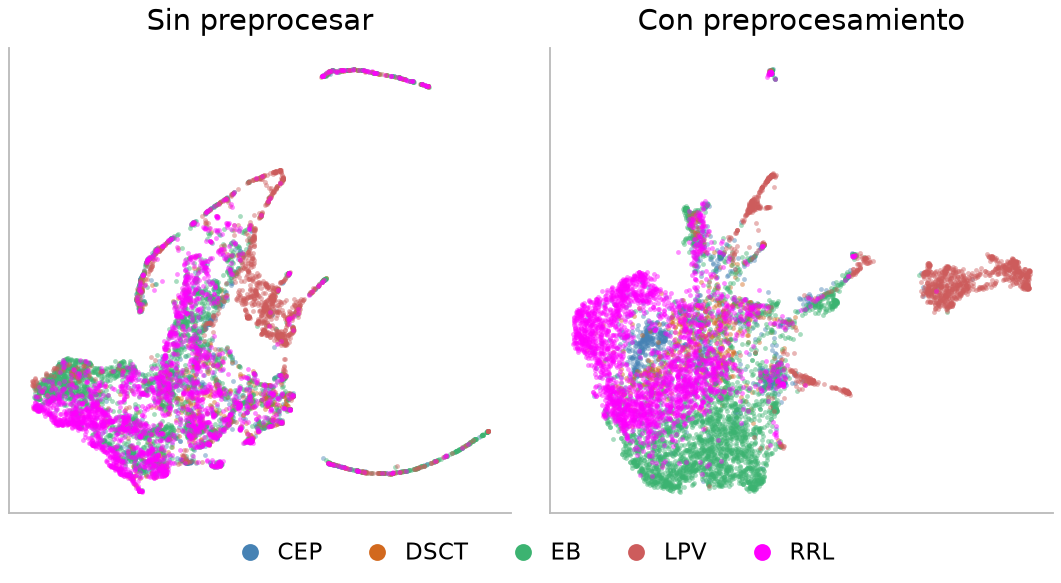
\includegraphics[width=\textwidth]{figures/umap_features.png}\\[0.1em]
{\scriptsize UMAP (\texttt{n\_neighbors} = 20) de las features de los 8.419 objetos.\\
Con el preprocesamiento LPV se separa y aparecen zonas por clase}
\end{column}
\end{columns}
\end{frame}

% ============================================================
\begin{frame}
\frametitle{Decisión 1: features, transformaciones y recorte}
\vspace{-0.5em}
\begin{columns}[T]
\begin{column}{0.53\textwidth}
{\small
\begin{itemize}\itemsep=3pt
\item \textbf{Se descartan 20 de 178}: 14 de no-detecciones previas a la primera alerta y 6
  colores WISE. Su dato faltante no es física de la estrella
\item \textbf{Verificación}: un random forest obtiene el mismo F1 macro con 158 features que
  con 178 (0,92)
\item \textbf{Logaritmo}: $\log_{10}$ a los tres períodos, que van de horas a cientos de días, y
  $\log(1+x)$ a 20 features positivas de cola larga
\item \textbf{Recorte de valores extremos}: cada feature se limita al rango entre sus
  percentiles 1 y 99 de train. Lo que queda fuera se reemplaza por el límite, sin eliminar
  objetos. Afecta al 1,8\,\% de los valores
\item \textbf{Después}: imputación con la mediana y z-score
\end{itemize}
}
\end{column}

\begin{column}{0.45\textwidth}
\centering
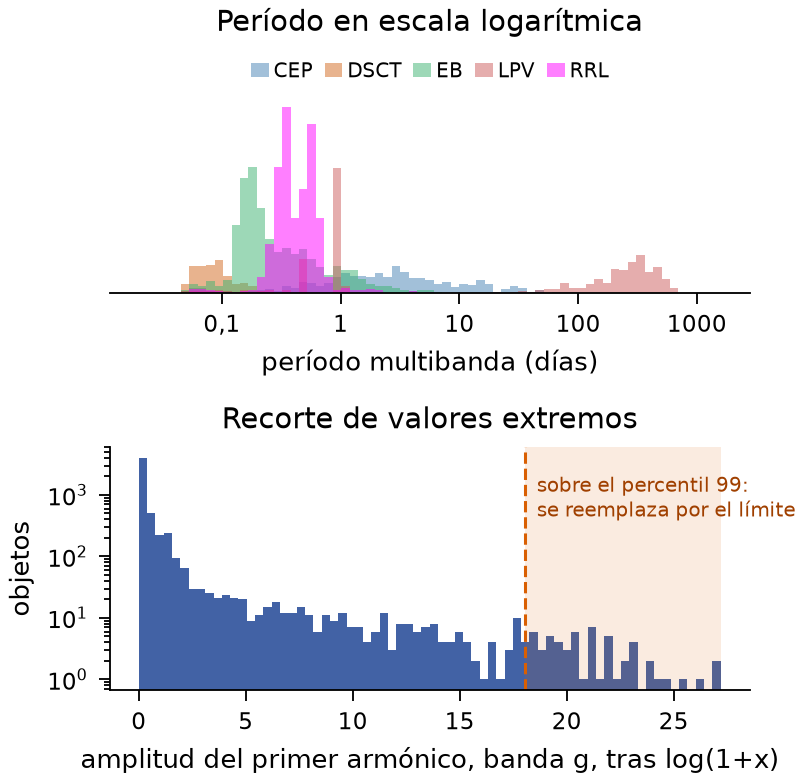
\includegraphics[width=0.96\textwidth]{figures/transformaciones.png}
\end{column}
\end{columns}
\end{frame}

% ============================================================
\begin{frame}
\frametitle{Decisión 2: normalización con z-score}
\vspace{-0.7em}
\begin{center}
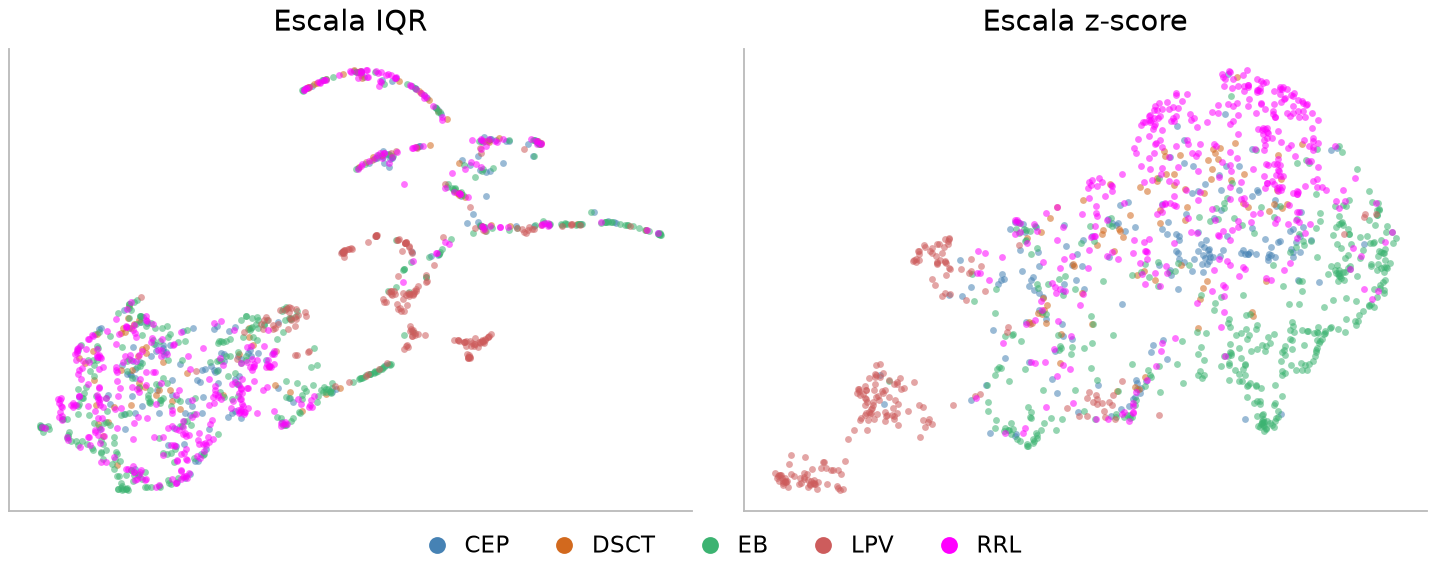
\includegraphics[width=0.63\textwidth]{figures/escala_latente.png}\\[-0.1em]
{\scriptsize Espacio latente del autoencoder en test, proyectado con UMAP
(\texttt{n\_neighbors} = 20) y coloreado por clase}
\end{center}
\vspace{-0.6em}
\begin{columns}[T]
\begin{column}{0.52\textwidth}
{\footnotesize
\begin{itemize}\itemsep=2pt
\item \textbf{Escala inicial}: mediana e IQR. En features de cola pesada quedan valores de
  hasta 300 y el autoencoder aprende esas, no el período
\item \textbf{Cambio}: z-score con media y desviación de train. Todas pesan lo mismo en el error
\end{itemize}
}
\end{column}

\begin{column}{0.45\textwidth}
\centering
{\footnotesize
\begin{tabular}{lcc}
\toprule
ARI en test & IQR & z-score \\
\midrule
Grupos del GMM      & 0,11 & \textbf{0,20} \\
Centros de MCDSVDD  & 0,36 & \textbf{0,69} \\
\bottomrule
\end{tabular}\\[0.3em]
}
\parbox{0.95\linewidth}{\centering\scriptsize \textbf{ARI}: cuánto coinciden los grupos del
modelo con las clases reales. 0 es azar y 1 es coincidencia perfecta}
\end{column}
\end{columns}
\end{frame}

% ============================================================
\begin{frame}
\frametitle{Metodología: del dato al cluster}
\vspace{-0.6em}
\begin{center}
\begin{tikzpicture}[
  stage/.style={draw=black, thick, rounded corners=1pt, align=center,
                execute at begin node={\hyphenpenalty=10000},
                text width=2.25cm, minimum height=0.95cm, font=\scriptsize, inner sep=3pt},
  modelo/.style={draw=structure, thick, rounded corners=1pt, align=center, text=structure,
                execute at begin node={\hyphenpenalty=10000},
                text width=2.55cm, minimum height=0.72cm, font=\scriptsize, inner sep=3pt},
  fl/.style={->, >=stealth, thick}]

  \node[stage] (d)                     {158 features\\ por estrella};
  \node[stage, right=0.30cm of d] (p)  {preprocesamiento\\ ajustado en train};
  \node[stage, right=0.30cm of p] (a)  {autoencoder\\ 512--256--128--\textbf{8}};
  \node[modelo, right=0.45cm of a, yshift=0.50cm]  (g) {GMM\\ sin etiquetas};
  \node[modelo, right=0.45cm of a, yshift=-0.50cm] (m) {MCDSVDD\\ con etiquetas};
  \node[stage, right=3.45cm of a] (c)  {curvas de luz:\\ prototipos y outliers};

  \draw[fl] (d) -- (p);
  \draw[fl] (p) -- (a);
  \draw[fl] (a.east) -- (g.west);
  \draw[fl] (a.east) -- (m.west);
  \draw[fl] (g.east) -- (c.west);
  \draw[fl] (m.east) -- (c.west);
\end{tikzpicture}
\end{center}
\vspace{-0.4em}
\begin{columns}[T]
\begin{column}{0.50\textwidth}
{\footnotesize
\begin{itemize}\itemsep=3pt
\item \textbf{Partición} 70/15/15 estratificada. Recorte, imputación y escala se ajustan solo
  con train: sin fuga de información
\item \textbf{Autoencoder}: MLP con BatchNorm y LeakyReLU, salida lineal, error cuadrático
  medio, Adam y \emph{early stopping} con validación
\item \textbf{Herramientas}: Python, PyTorch, scikit-learn y umap-learn. Código con pruebas
  en GitHub
\end{itemize}
}
\end{column}

\begin{column}{0.47\textwidth}
\centering
{\footnotesize \textbf{Decisión 3: tamaño del cuello de botella}}\\[0.25em]
{\scriptsize \setlength{\tabcolsep}{3pt}
\begin{tabular}{cccc}
\toprule
Dimensión & Error (MSE) & ARI GMM & ARI MCDSVDD \\
\midrule
2  & 0,54 & 0,13 & 0,55 \\
4  & 0,42 & 0,20 & 0,77 \\
\textbf{8} & 0,34 & 0,21 & \textbf{0,80} \\
16 & 0,26 & 0,23 & 0,79 \\
32 & 0,21 & 0,33 & 0,78 \\
\bottomrule
\end{tabular}\\[0.4em]
\parbox{0.97\linewidth}{\centering\scriptsize \textbf{ARI}: coincidencia de los grupos con las
clases reales (0 es azar, 1 es perfecta), en validación y promediando 3 semillas. Con menos de
8 se pierde información y 8 es el máximo de MCDSVDD}
}
\end{column}
\end{columns}
\end{frame}
